	\section{Use case: Spaces}
	\subsection{Use case diagram}
	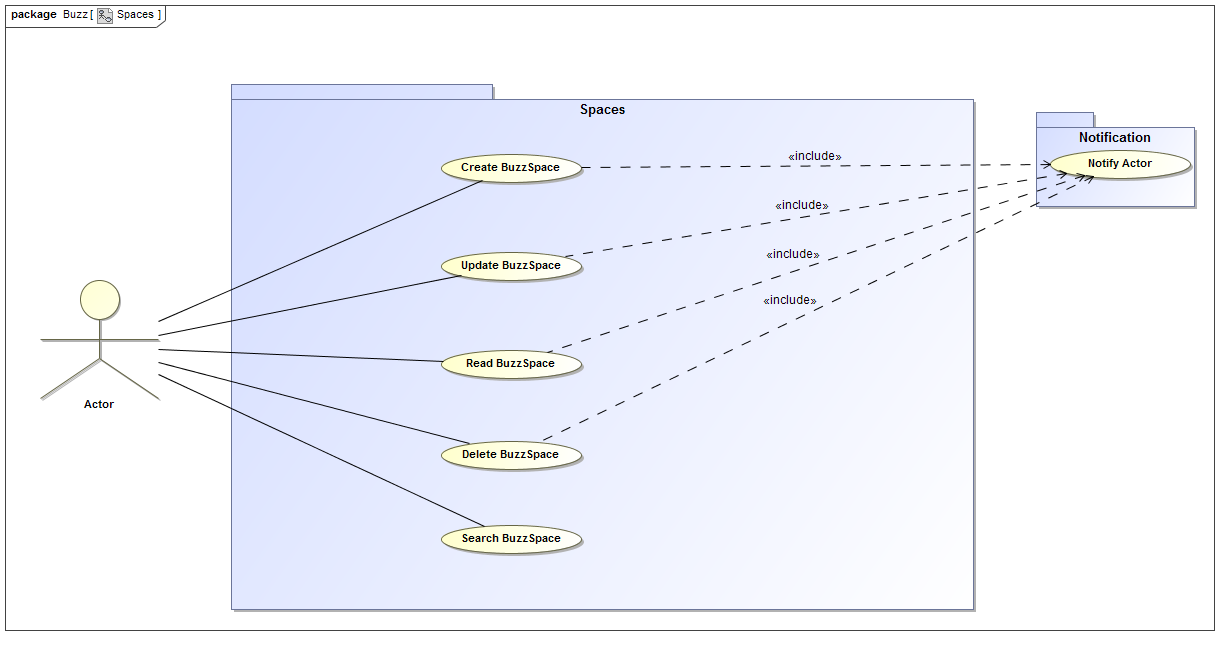
\includegraphics[width=\textwidth]{spacesUseCase}
	\subsection{Short description}
	\begin{description}
		
		\item[] 
			The following section will discuss the functional requirements of the Spaces section of the BuzzSpace program.
		
		\item[] Different actors:
		\begin{itemize}
			\item Administrator: Has system wide permission.
			\item Lecturer: Has full permission for the current BuzzSpace
			\item User: Has permission for the current BuzzSpace according to the users XP. Lecturer will included in users as they will be assigned the required XP.   
		\end{itemize}
		
	\end{description}
	
	\subsection{Use case prioritization}
	\begin{description}
		\item[] Critical
		\begin{itemize}
			\item Create BuzzSpace
			\item Delete BuzzSpace
			\item Update BuzzSpace
			\item Read BuzzSpace
			\item Authentication
		\end{itemize}
		
		\item[] Important
		\begin{itemize}
			\item Search BuzzSpaces
			\item Check XP
		\end{itemize}
	\end{description}
	
	\subsection{Use cases}
	\newpage
	\begin{longtable}{@{}|p{1.5cm}|p{2.2cm}|p{3cm}|p{3.5cm}|p{3.5cm}|@{}}
		\toprule
		\multicolumn{5}{|c|}{\textbf{Use cases for Space}}\\
		\hline
		\textbf{Actor} & \textbf{Use Case} & \textbf{Pre-condition} & \textbf{Post-Conditions} & \textbf{Description} \\ \midrule
		
		User Or Admin& 
		Create BuzzSpace& 
		\begin{itemize}
			\item A group must exist
			\item The actor has permission
			\item The actor has the required amount of XP
		\end{itemize}& 
		\begin{itemize}
			\item Space created
		\end{itemize} & 
		Create a new BuzzSpace (discussion space within group) \\ \midrule
		
		User Or Admin& 
		Delete BuzzSpace& 
		\begin{itemize}
			\item The BuzzSpace exists that wants to be removed
			\item The actor has permission
			\item The actor has the required amount of XP
		\end{itemize}& 
		\begin{itemize}
			\item BuzzSpace removed from groups
		\end{itemize} & 
		Remove a BuzzSpace from groups and notify the users belonging to that group \\ \midrule
		
		User Or Admin& 
		Update BuzzSpace& 
		\begin{itemize}
			\item The Space exists that needs to be updated
			\item The actor has permission
			\item The actor has the required amount of XP
		\end{itemize}& 
		\begin{itemize}
			\item State of space changed
		\end{itemize} & 
		Allow users with permission to update the BuzzSpace \\ \midrule
		
		User Or Admin& 
		Read BuzzSpace& 
		\begin{itemize}
			\item The Space exists
			\item The actor has permission
		\end{itemize}& 
		\begin{itemize}
			\item BuzzSpace marked read
		\end{itemize} & 
		Allow users with permission to read the BuzzSpaces \\ \midrule
		
		User Or Admin& 
		Search BuzzSpaces& 
		\begin{itemize}
			\item Must be a registered user
		\end{itemize}& 
		\begin{itemize}
			\item Search list created
		\end{itemize} & 
		Search the BuzzSpaces in groups \\ \midrule
		
		User Or Admin& 
		Authentication& 
		\begin{itemize}
			\item Actor must be registered
			\item Actor must be logged into the Buzz System 
		\end{itemize}& 
		\begin{itemize}
			\item Actor grated access
		\end{itemize} & 
		See if the Actor is authenticated to the system \\ \midrule
		
		User Or Admin& 
		Check XP& 
		\begin{itemize}
			\item Actor must be registered
			\item Actor must be logged into the Buzz System 
			\item Actor has the required amount of XP
		\end{itemize}& 
		\begin{itemize}
			\item Actor allowed to make changes
		\end{itemize} & 
		See if the Actor has the required amount of XP to be allowed to make changes to the BuzzSpace \\ \bottomrule
		
	\end{longtable}